%*******************************************************************************
%*********************************** First Chapter *****************************
%*******************************************************************************

\chapter{Tổng quan}  %Title of the First Chapter

\ifpdf
    \graphicspath{{Chapter1/Figs/Raster/}{Chapter1/Figs/PDF/}{Chapter1/Figs/}{}}
\else
    \graphicspath{{Chapter1/Figs/Vector/}{Chapter1/Figs/}}
\fi


%********************************** %First Section  **************************************
\section{Mở đầu} %Section - 1.1 
\subsection{Mục đích đề tài và tính cấp bách}
Trong cuộc sống bận rộn hiện nay, con người chúng ta hay có xu hướng bị xao nhãng và bỏ quên các thiết bị nhỏ. trong đó có thiết bị điện thoại di động và chùm chìa khóa là hai vật rất quan trọng và thường hay bỏ quên nhất. Và tìm kiếm chúng không hề dễ dàng, nhất là khi đang vội thì sẽ làm mọi thứ rối tung lên.

Và đồng thời hiện nay công nghệ phát triển cho các thiết bị kết nối không dây phát triển mạnh, có thể ứng dụng cho nhiều lĩnh vực. Bluetooth Low Energy là một trong những cái tên nổi bật nhất trong các công nghệ truyền dữ liệu không dây bởi đặc tính tiện lợi, phổ biến và tiết kiệm năng lượng. Và nhóm chúng tôi muốn tìm hiểu và ứng dụng công nghệ này vào cuộc sống thực tiễn.

Từ điều đó đã thúc đẩy nhóm chúng tôi tìm cách giải quyết và nảy ra ý tưởng tạo ra sản phẩm móc khóa thông mình - Smart Keyring có chức năng kết nối với thiết bị di động sử dụng công nghệ BLE để giải quyết vấn đề trên dựa trên các tính năng của BLE.
\subsection{Mô tả đề tài}

Đề tài sẽ chia làm 2 phần chính:

• \textbf{Sản phẩm móc khóa}: 1 thiết bị có kích thước nhỏ, năng lượng tiêu thụ ít. 

Chức năng:

- Báo hiệu bằng âm thanh và ánh sáng khi có yêu cầu định vị.

- Điều khiển chức năng định vị trên thiết bị di động qua nút ấn.
	
- Báo hiệu khi mất kết nối với thiết bị di động.
		

• \textbf{Ứng dụng di động}: ứng dụng chạy trên nền tảng Android. 

Chức năng:

- Gửi yêu cầu định vị tới sản phẩm móc khóa để kích hoạt tính năng báo hiệu trên móc khóa.

- Báo hiệu bằng âm thanh yêu cầu định vị.

- Báo hiệu khi bị mất kết nối với sản phẩm móc khóa.

\subsection{Tình hình nghiên cứu}

• Tình hình nghiên cứu ngoài nước:

- Thiết bị \href{www.thetrackr.com}{TrackR} 
(\url{www.thetrackr.com}) : sử dụng công nghệ Bluetooth Low Energy, có chức năng tìm kiếm thiết bị và chống thất lạc để quên. Tuy nhiên hạn chế là chưa phân phối chính thức ở Việt Nam và giá thành còn khá cao so với mức sống của người Việt Nam.

• Tình hình nghiên cứu trong nước:

- Chưa thấy xuất hiện sản phẩm có chức năng tương tự sử dụng công nghệ BLE.

- Có vài sản phẩm có chức năng gần giống sử dụng 2 thẻ tag RF để tìm nhau, chưa có chức năng cảnh báo khi mất kết nối (trường hợp để quên hoặc trộm mất)

- Chưa có tài liệu nghiên cứu về lập trình trên hệ thống System on Chip, chỉ có hướng dẫn sử dụng module theo firmware sẵn có từ nhà sản xuất. Cần tìm hiểu và nghiên cứu, so sánh về tính ứng dụng giữa 2 hướng phát triển trên. 

\subsection{Mục tiêu - Phạm vi - Đối tượng nghiên cứu}

Xuất phát từ các lý do trình bày ở trên, chúng tôi đã thực hiện đề tài “Thiết kế sản phẩm móc khóa thông minh (Smart Keyring) dựa trên nền tảng công nghệ Bluetooth Low Energy (BLE)”. Mục tiêu của đề tài là:

• Tìm hiểu về công nghệ Bluetooth Low Energy

• Kế thiết bị “Móc khóa thông minh - SmartKeyring” sử dụng công nghệ

Bluetooth và kết nối với ứng dụng Android trên điện thoại.

\nomenclature[z-cif]{$CIF$}{Cauchy's Integral Formula}                                % first letter Z is for Acronyms 
\nomenclature[a-F]{$F$}{complex function}                                                   % first letter A is for Roman symbols
\nomenclature[g-p]{$\pi$}{ $\simeq 3.14\ldots$}                                             % first letter G is for Greek Symbols
\nomenclature[g-i]{$\iota$}{unit imaginary number $\sqrt{-1}$}                      % first letter G is for Greek Symbols
\nomenclature[g-g]{$\gamma$}{a simply closed curve on a complex plane}  % first letter G is for Greek Symbols
\nomenclature[x-i]{$\oint_\gamma$}{integration around a curve $\gamma$} % first letter X is for Other Symbols
\nomenclature[r-j]{$j$}{superscript index}                                                       % first letter R is for superscripts
\nomenclature[s-0]{$0$}{subscript index}                                                        % first letter S is for subscripts

%TODO: BLE bỏ ở đây có hợp lý không?
%********************************** % Third Section  *************************************
\section{Bluetooth Low Energy (BLE) }  %Section - 1.3 
\label{section1.3} 
Khái niệm BLE xuất hiện từ phiên bản 4.0, là một bước ngoặc lớn trong sự phát triển kết nối không dây. Các mạch BLE rất nhỏ cùng với công suất tiêu thụ hiệu năng cực thấp (khoảng vài chục uA khi hoạt động), nên hầu hết các thiết bị đều có thể tích hợp công nghệ này, từ các thiết bị nhỏ bé như tai nghe, chìa khóa.. cho tới các thiết bị lớn như tủ lạnh, tivi, xe máy... Nhờ đó, các thiết bị có thể trở nên "smart".\cite{hte}
\begin{figure}[H]
	\centering    
	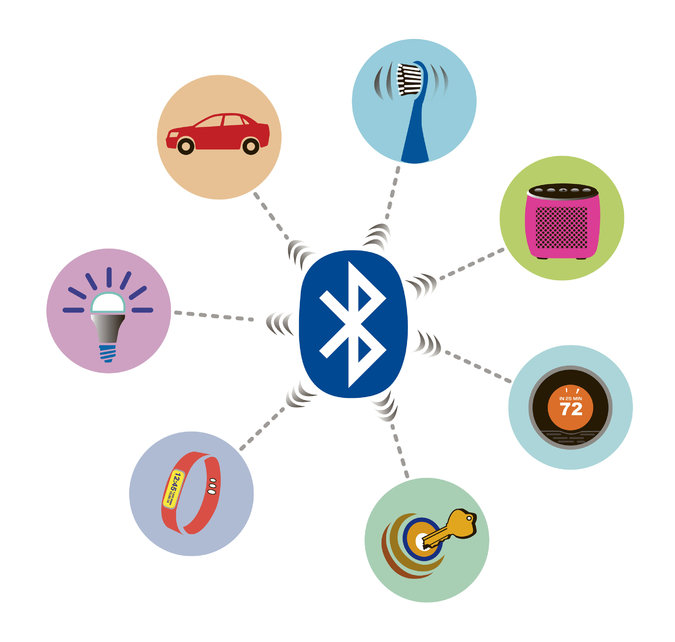
\includegraphics[width=0.7\textwidth]{btuse}
	\caption[Các ứng dụng Bluetooth]{Các ứng dụng Bluetooth}
	\label{fig:btuse}
\end{figure}
\subsection{Khái niệm và lịch sử phát triển Bluetooth}
Bluetooth là công nghệ không dây cho phép các thiết bị điện, điện tử giao tiếp với nhau trong khoảng cách ngắn, bằng sóng vô tuyến qua băng tần chung ISM (Industrial, Scientific, Medical) trong dãy tầng 2.40- 2.48 GHz. Đây là dãy băng tầng không cần đăng ký được dành riêng để dùng cho các thiết bị không dây trong công nghiệp, khoa học, y tế.

	\begin{table}[ht]
		\begin{tabular}{ |c|m{2cm}|m{2cm}|m{2cm}|m{2cm}| } 
			\hline
			& \textbf{Bluetooth} & \textbf{BLE} & \textbf{Wifi} & \textbf{Zigbee} \\ 
			\hline
			\textbf{Radio Frequency} &	2.4G &	2.4G &	2.4G &	2.4G \\ 
			\hline
			\textbf{Distance Range} &	10m	&>60m &	30m	& 10-100m \\ 
			\hline
			\textbf{Air Datarate} &	1-3Mbps &	1Mbps &	54Mbps &	250kbps \\
			\hline
			\textbf{Application Throughput} &	0.7-2.1Mbps &	305kbps &Depend &120kbps\\
			\hline
			\textbf{Security} &	64bit, 128bit &	128-bit & AES	SSID, WEP&	128-bit AES \\
			\hline
			\textbf{Power consumption}&	Low	&Very Low&	High&	Low \\
			\hline
			\textbf{Certification Body}&	Bluetooth SIG&	Bluetooth SIG&	IEEE802.11&	IEEE802.15.4 \\
			\hline
			\textbf{Network topology} &	Point-to-Point Scatternet&	Point-to-Point Star&	Point-to-Hub& 		Mesh, Ad-hoc\\
			\hline
		\end{tabular}
		\caption {Bảng so sánh các công nghệ truyền không dây}
		\label{table:1.1}
	\end{table}


Lịch sử phát triển: \cite{tgdd}

•Bluetooth 4.0 - Bluetooth Low Energy: Là sự kết hợp của các đời Bluetooth trước đó với nhau. Bluetooth 4.0 đạt tốc độ truyền tải lên đến 25Mbps, dễ dàng ghép đôi các thiết bị với nhau, hiệu năng tiêu thụ thấp. Đây là chuẩn Bluetooth được sử dụng trên hầu hết các thiết bị hiện nay.

•Bluetooth 4.1 và 4.2: Là phiên bản ra đời đầu năm 2014 với nhiều cải tiến vượt bậc so với Bluetooth 4.0 như khả năng điều chống chồng chéo tín hiệu, kết nối thực sự thông minh và khả năng truyền dữ liệu độc lập mà không cần phụ thuôc vào trung tâm điều khiển. Phiên bản 4.2 được phát triển có khả năng truyền tải cao và bảo mật hơn, nhưng quan trọng hơn cả là cho phép các vi xử lý sử dụng chuẩn giao thức Ipv6 để truy cập trực tiếp vào internet.

•Bluetooth 5.0: theo dự kiến sẽ bắt đầu xuất hiện trên các thiết bị thương mại vào cuối 2016 nay hoặc đầu năm 2017 (Q1). Bluetooth 5.0 có tầm phủ sóng tăng lên gấp 4 lần so với Bluetooth 4.2 hiện nay, còn tốc độ truyền dữ liệu thì tăng lên cao nhất là 2 lần. Việc mở rộng khả năng phủ sóng của Bluetooth sẽ giúp các thiết bị Internet of Things sẽ có thể giao tiếp với nhau cũng như với trạm điều khiển một cách dễ dàng hơn, vượt qua bức tường của một căn nhà bình thường, trong khi lại tăng tốc thu thập và truyền dữ liệu. Chuẩn Bluetooth mới cũng sẽ giúp các beacon và giải pháp nhận diện địa điểm trở nên thông minh, chính xác và phản hồi nhanh hơn với sự hiện diện của người dùng.

\subsection{Phân loại vai trò thiết bị BLE}
Có 4 loại thiết bị BLE (có thể gọi là chế độ hoạt động) đó là Peripheral, Central, Observer và Broadcaster và bình thường thì một thiết bị BLE chỉ hoạt động  trong một chế độ.

• \textbf{Central} là thiết bị sẽ chủ động yêu cầu kết nối đến các thiết bị BLE khác (thường là smartphone, tablet). Sau khi kết nối thì chúng ta lại gọi BLE Central là  BLE Master.

• \textbf{BLE Peripheral} là thiết bị chấp nhận yêu cầu kết nối (thường là đồ vật BLE). Tương tự, sau khi kết nối thì chúng ta gọi BLE Peripheral là BLE Slave.

• \textbf{BLE Observer} là BLE Central nhưng chỉ nhận dữ liệu nhận dạng của các thiết bị xung quanh nhưng không bao giờ tạo kết nối

• \textbf{BLE Broadcaster} là BLE Peripheral chỉ phát dữ liệu nhận dạng nhưng không bao giờ chấp nhận yêu cầu kết nối từ các BLE Central.
 
\subsection{Cách thức hoạt động của BLE}
Theo chuẩn BLE định nghĩa thì các thiết bị BLE có 4 hoạt động cơ bản như sau: \cite{hte}

• \textbf{Advertising}: là hoạt động phát dữ liệu nhận dạng cơ bản của thiết bị BLE Peripheral ra môi trường xung quanh trước khi kết nối

• \textbf{Scanning}: là hoạt động của thiết bị BLE Central để thu thập dữ liệu nhận dạng của nhiều thiết bị BLE Peripheral xung quanh

• \textbf{Connecting}: là hoạt động của cả thiết bị BLE Central và BLE peripheral trong đó thiết bị BLE Central có thể gửi yêu cầu thêm thông tin nhận dạng (gọi là Scan Request) và BLE Peripheral gửi theo yêu cầu (gọi là Scan Response). Sau đó BLE Central sẽ kiểm tra đầy đủ thông tin nhận dạng (từ Advertising data và từ Scan Response data) và gửi yêu cầu kết nối (gọi là Connection Request), cuối cùng thiết bị BLE Peripheral sẽ trả lời chấp nhận hay từ chối kết nối (gọi là Connection Response)

• \textbf{Discovering}: là hoạt động của thiết bị BLE Client sau khi kết nối nhằm lấy thông tin về các loại dữ liệu mà thiết bị BLE Server có thể cung cấp. Ví dụ, thiết bị BLE Server có thể có dữ liệu về gia tốc, hoặc có dữ liệu về nhiệt độ, độ ẩm, v.v.. và thiết bị BLE Client sẽ có nhu cầu biết các loại dữ liệu nào có thể nhận từ BLE Server

Cách thức hoạt động của BLE ở hình \ref{fig: btwork}:
	\begin{figure}[h]
		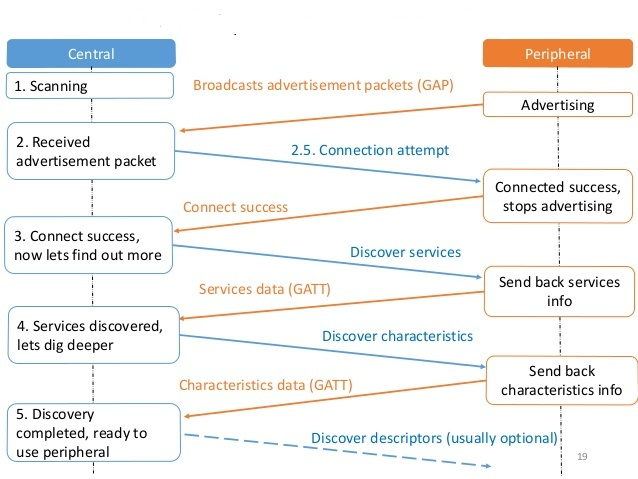
\includegraphics[width=1.0\textwidth]{btwork}
		\caption[Sơ đồ hoạt động của BLE]{Sơ đồ hoạt động của BLE}
		\label{fig: btwork}
	\end{figure}
	
\newpage
\subsection{Các vi điều khiển tích hợp công nghệ BLE}
Các SoC tích hợp sẵn công nghệ BLE phố biến có thể kể đến:

• Texas Instruments: CC2540/CC2541, dòng CC256x, CC26xx

• Nordic Semiconductor: nRF51822, nRF8001

• CSR CSR101x

• Cypress Semiconductor PSoC 4 BLE / PRoC BLE

Tuy nhiên ở Việt Nam tại thời điểm bắt đầu nghiên cứu và hiện thực đề tài thì 2 loại chipset phổ biến và có giá tiền phổ thông là CC2540 và CC2541 được cung cấp theo dạng Module HM-10.
	\begin{figure}[h]
		\centering    
		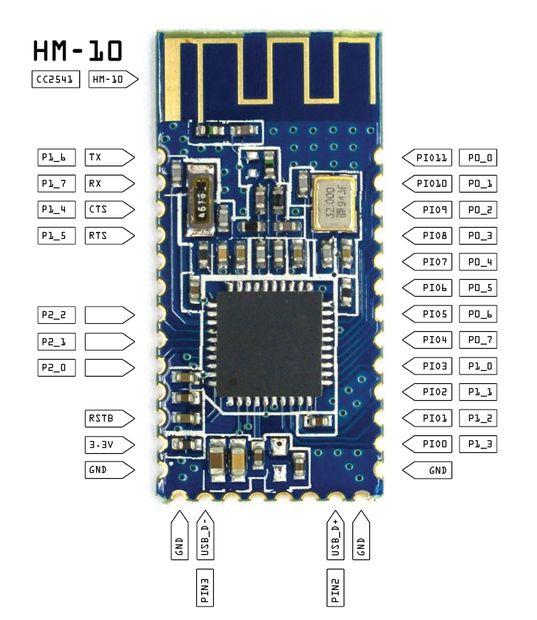
\includegraphics[width=0.4\textwidth]{hm10}
		\caption[Module HM-10]{Module HM-10}
		\label{fig: hm10}
	\end{figure}

\nomenclature[z-FEM]{FEM}{Finite Element Method}
\nomenclature[z-PFEM]{PFEM}{Particle Finite Element Method}
\nomenclature[z-FVM]{FVM}{Finite Volume Method}
\nomenclature[z-BEM]{BEM}{Boundary Element Method}
\nomenclature[z-MPM]{MPM}{Material Point Method}
\nomenclature[z-LBM]{LBM}{Lattice Boltzmann Method}
\nomenclature[z-MRT]{MRT}{Multi-Relaxation 
Time}
\nomenclature[z-RVE]{RVE}{Representative Elemental Volume}
\nomenclature[z-GPU]{GPU}{Graphics Processing Unit}
\nomenclature[z-SH]{SH}{Savage Hutter}
\nomenclature[z-CFD]{CFD}{Computational Fluid Dynamics}
\nomenclature[z-LES]{LES}{Large Eddy Simulation}
\nomenclature[z-FLOP]{FLOP}{Floating Point Operations}
\nomenclature[z-ALU]{ALU}{Arithmetic Logic Unit}
\nomenclature[z-FPU]{FPU}{Floating Point Unit}
\nomenclature[z-SM]{SM}{Streaming Multiprocessors}
\nomenclature[z-PCI]{PCI}{Peripheral Component Interconnect}
\nomenclature[z-CK]{CK}{Carman - Kozeny}
\nomenclature[z-CD]{CD}{Contact Dynamics}
\nomenclature[z-DNS]{DNS}{Direct Numerical Simulation}
\nomenclature[z-EFG]{EFG}{Element-Free Galerkin}
\nomenclature[z-PIC]{PIC}{Particle-in-cell}
\nomenclature[z-USF]{USF}{Update Stress First}
\nomenclature[z-USL]{USL}{Update Stress Last}
\nomenclature[s-crit]{crit}{Critical state}
\nomenclature[z-DKT]{DKT}{Draft Kiss Tumble}
\nomenclature[z-PPC]{PPC}{Particles per cell}